% Dmitry Mikushin, USI Lugano, dmitry.mikushin@usi.ch,
% using portions of original style file by Tom Cashman
%
% IMPORTANT NOTICE:
%
% The USI logo is unique; it is authorized for use only by employees of the
% Università della Svizzera italiana for work-related projects; others can use them
% ONLY with prior authorization (contact: press@usi.ch).
%
% http://www.press.usi.ch/en/corporate-design/corporate-design-stampa.htm
%
% This is an example beamer presentation, which uses Università della Svizzera italiana
% design theme.

\documentclass[aspectratio=169]{beamer}

\usetheme{usi}

\usepackage{multirow}
\usepackage{hhline}
\usepackage{tikz}
\usetikzlibrary{shapes.geometric}

\lstdefinelanguage{shuffle}
{
morekeywords={if,__shfl_up,laneid,float},
}

\newcommand\score[2]{
\pgfmathsetmacro\pgfxa{#1+1}
\tikzstyle{scorestars}=[star, star points=5, star point ratio=2.25, draw,inner sep=1.3pt,anchor=inner point 3]
  \begin{tikzpicture}[baseline]
    \foreach \i in {1,...,#2} {
    \pgfmathparse{(\i<=#1?"usi@yellow":"gray")}
    \edef\starcolor{\pgfmathresult}
    \draw (\i*2.0ex,0) node[name=star\i,scorestars,fill=\starcolor,color=\starcolor]  {};
   }
  \end{tikzpicture}
}

\setlength{\fboxsep}{0.25pt}%
\setlength{\fboxrule}{0pt}%

\title[GPU parallelizing compiler]{Evaluating manual and compiler-driven parallelization\\ of stencil micro-applications on a GPU-enabled cluster}
\author{Dmitry Mikushin, Olaf Schenk}
\institute{}
\date{February 21, 2014}



\begin{document}
\begin{frame}
\titlepage
\end{frame}



\begin{frame}[fragile]{Annotation}

\begin{minipage}{15cm}
In this talk we will demonstrate how parallelization and further optimization of stencil codes for GPUs could be automated by compiler toolchains. By example of wave equation stencil, hand-written naive and optimized for locality versions will be compared against compiler-generated parallel code, presenting the roofline performance, efficiency of tiling, JIT-compilation and other properties. The results of benchmarking KernelGen and PPCG auto-parallelizing compilers as well as one commercial OpenACC compiler will be presented on a set of 10 stencil micro-applications.% Finally, we will show how automatically parallelized code of a very large wave propagation problem performs on the Pitz Daint supercomputer.
\end{minipage}

\end{frame}



\begin{frame}[fragile]{3D Finite Difference Computation on GPUs using CUDA}

\begin{minipage}{8.5cm}
A famous \href{http://developer.download.nvidia.com/CUDA/CUDA_Zone/papers/gpu_3dfd_rev.pdf}{paper} by Paulius Micikevicius, \textbf{280} citations:
\vskip5pt
\begin{itemize}
\item Stencil for 3D wave equation ($6$-$12^{th}$ order in space, $2^{nd}$ order in time)
\item 2D slices are tiled in GPU shared memory
\item Columns of $3^{rd}$ dimension are cached in GPU thread registers
\item Released in 2009, performance tested on Tesla S1060 (GT200)
\end{itemize}
\end{minipage}%
\hskip0.5cm
\begin{minipage}{6cm}
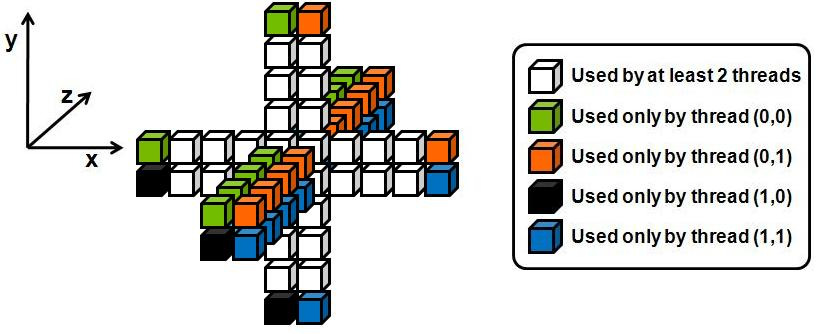
\includegraphics[width=6cm]{figures/paulius_fig2}
\vskip10pt
\hskip3.85cm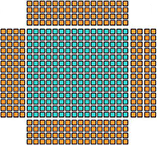
\includegraphics[width=2cm]{figures/paulius_fig1}
\end{minipage}

\end{frame}



\begin{frame}[fragile]{Questions we addressed in this study}

\begin{enumerate}
\item Are those frequently cited tiling optimizations still beneficial on modern GPUs?
\item Are there any new stencil-related optimizations yet to discover?
\item To what extent the generation of GPU kernels for stencils could be automated?
\begin{itemize}
\item Can compilers generate \emph{efficient} parallel GPU code for stencils?
\item What manual optimizations could be easily implemented by compiler?
\end{itemize}
\end{enumerate}

\end{frame}



\begin{frame}[fragile]{Example wave 3D stencil}

\begin{lstlisting}[language=c]
for (int k = 2; k < ns - 2; k++)
    for (int j = 2; j < ny - 2; j++)
        for (int i = 2; i < nx - 2; i++)
        {
                w2[k][j][i] =  m0 * w1[k][j][i] - w0[k][j][i] +

                    m1 * (
                        w1[k][j][i+1] + w1[k][j][i-1]  +
                        w1[k][j+1][i] + w1[k][j-1][i]  +
                        w1[k+1][j][i] + w1[k-1][j][i]) +
                    m2 * (
                        w1[k][j][i+2] + w1[k][j][i-2]  +
                        w1[k][j+2][i] + w1[k][j-2][i]  +
                        w1[k+2][j][i] + w1[k-2][j][i]);
	}
\end{lstlisting}

{\small input: \emph{w0} (1 pt/iter), \emph{w1} (13 pt/iter)\\
output: \emph{w2} (1 pt/iter)}

\end{frame}



\begin{frame}[fragile,t]{Reproducing P. Micikevicius method for wave13pt \underline{on S1070}}

\begin{minipage}[t][2.5cm]{\textwidth}
\begin{itemize}
\item $\{32, 16, 1\}$ blocks, maxrregcount=32
\item each thread is handling points of the same vertical column
\item array items reusable by the next point are tiled in registers
\item \emph{naive} -- na\"{i}ve CUDA version, \emph{shmem2dreg1d} -- with above optmzns applied
\item \emph{shmem2dreg1d} is almost \textbf{3$\times$} faster than \emph{naive} on S1070 -- \underline{remember this result!}
\end{itemize}
\end{minipage}

\begin{tikzpicture}[overlay] 
\node [xshift=0cm,yshift=0cm] at (7.45cm,-2cm)
{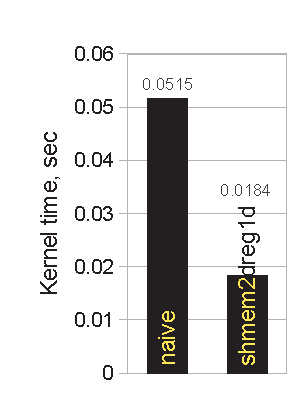
\includegraphics[width=2.4cm]{figures/wave13pt_time_s1070}};
\node [xshift=0cm,yshift=0cm] at (7.45cm,-3.85cm)
{\scriptsize \texttt{wave13pt} on Tesla S1070 (GT200/SM\_13), single precision};
\end{tikzpicture}%
\end{frame}



\begin{frame}[fragile,t]{Na\"{\i}ve CUDA implementation}

\begin{minipage}[t][2.5cm]{\textwidth}
\begin{itemize}
\item[]
\item $\{128, 1, 1\}$ blocks
\item one grid point per thread
\item[]
\end{itemize}
\end{minipage}

\begin{tikzpicture}[overlay] 
\node [xshift=0cm,yshift=0cm] at (7.45cm,-2cm)
{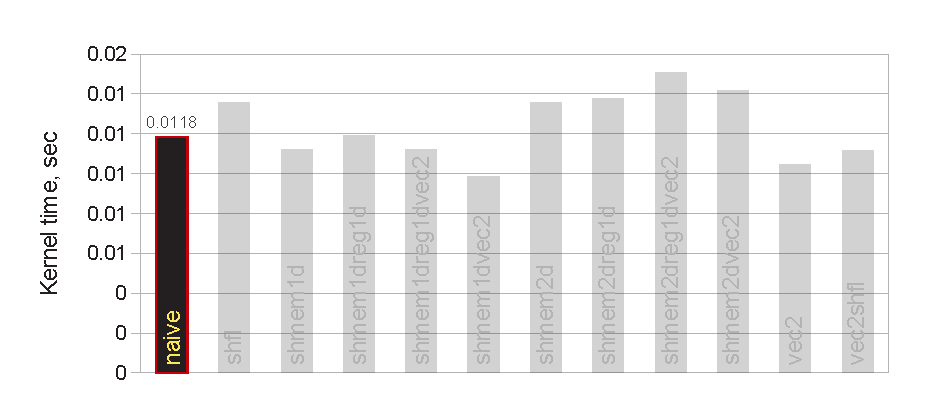
\includegraphics[width=7.5cm]{figures/wave13pt_time_01}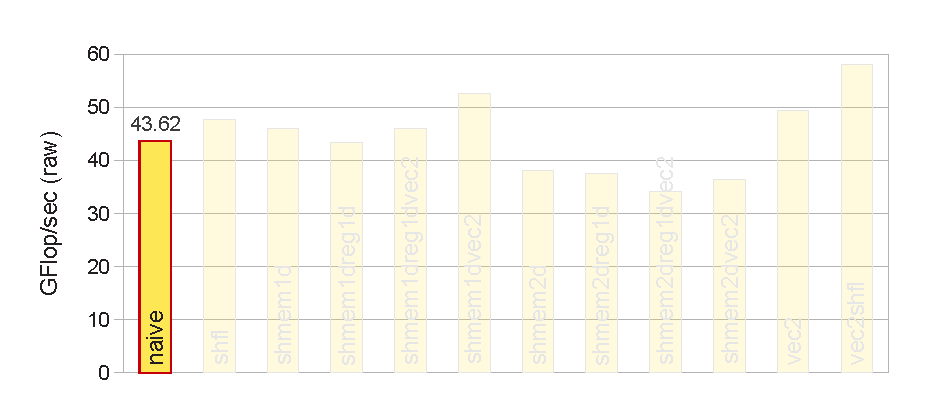
\includegraphics[width=7.5cm]{figures/wave13pt_gflops_01}};
\node [xshift=0cm,yshift=0cm] at (7.45cm,-3.85cm)
{\scriptsize \texttt{wave13pt} on GeForce GTX 680M (GK104/SM\_30), single precision};
\end{tikzpicture}%
\end{frame}



\begin{frame}[fragile,t]{Warp data shared with \emph{shuffle} instruction}

\begin{minipage}[t][2.5cm]{\textwidth}
\begin{itemize}
\item $\{128, 1, 1\}$ blocks
\item maxrregcount=32
\item load array value, use and pass to neighboring thread
\item shuffles are accounted into FLOPS, hence more FLOPS, but larger kernel time
\item \textcolor{blue}{needs shareable flops to be beneficial}
\end{itemize}
\end{minipage}

\begin{tikzpicture}[overlay] 
\node [xshift=0cm,yshift=0cm] at (7.45cm,-2cm)
{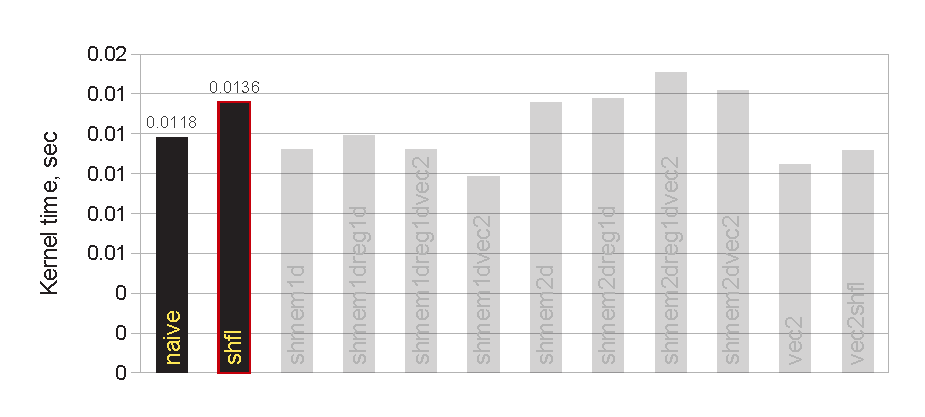
\includegraphics[width=7.5cm]{figures/wave13pt_time_02}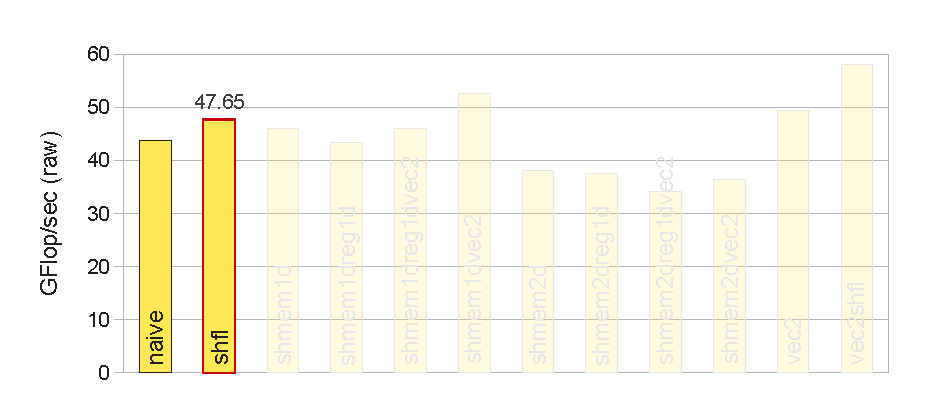
\includegraphics[width=7.5cm]{figures/wave13pt_gflops_02}};
\node [xshift=0cm,yshift=0cm] at (7.45cm,-3.85cm)
{\scriptsize \texttt{wave13pt} on GeForce GTX 680M (GK104/SM\_30), single precision};
\end{tikzpicture}%

\begin{tikzpicture}[overlay] 
\node [xshift=0cm,yshift=0cm] at (11.65cm,2.05cm)
{\begin{minipage}{5.8cm}\begin{lstlisting}[language=shuffle, basicstyle=\scriptsize]
float val = w1[k][j][i+2];
float result = m2 * val;
val = __shfl_up(val, 1);
if (laneid == 0) val = w1[k][j][i+1];
\end{lstlisting}\end{minipage}};
\end{tikzpicture}

\end{frame}



\begin{frame}[fragile,t]{Tiling 1D line of \emph{w1} array in shmem}

\begin{minipage}[t][2.5cm]{\textwidth}
\begin{itemize}
\item[]
\item[]
\item $\{128, 1, 1\}$ blocks
\item maxrregcount=32
\item[]
\item[]
\end{itemize}
\end{minipage}

\begin{tikzpicture}[overlay] 
\node [xshift=0cm,yshift=0cm] at (7.45cm,-2cm)
{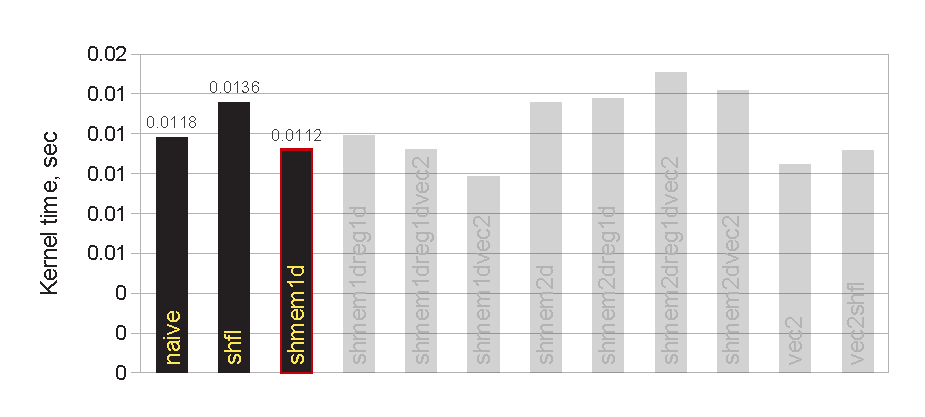
\includegraphics[width=7.5cm]{figures/wave13pt_time_03}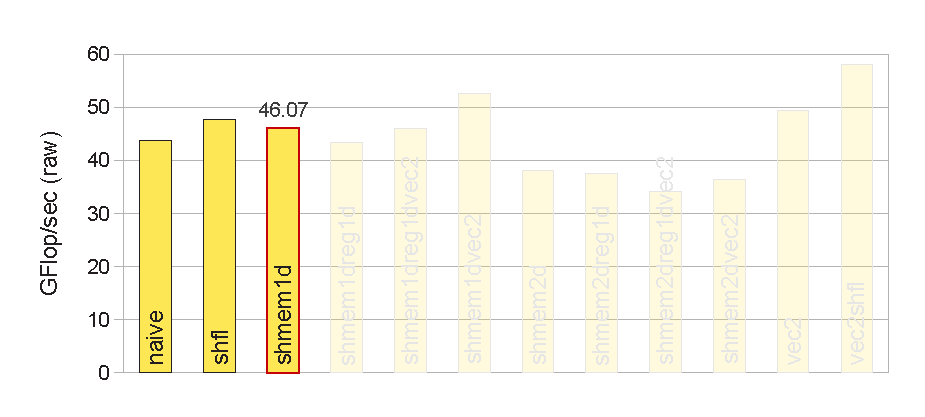
\includegraphics[width=7.5cm]{figures/wave13pt_gflops_03}};
\node [xshift=0cm,yshift=0cm] at (7.45cm,-3.85cm)
{\scriptsize \texttt{wave13pt} on GeForce GTX 680M (GK104/SM\_30), single precision};
\end{tikzpicture}%
\end{frame}



\begin{frame}[fragile,t]{Tiling 1D line of \emph{w1} array in shmem, vertical line in registers}

\begin{minipage}[t][2.5cm]{\textwidth}
\begin{itemize}
\item $\{128, 1, 1\}$ blocks
\item maxrregcount=32
\item each thread is handling points of the same vertical column
\item array items reusable by the next point are tiled in registers
\end{itemize}
\end{minipage}

\begin{tikzpicture}[overlay] 
\node [xshift=0cm,yshift=0cm] at (7.45cm,-2cm)
{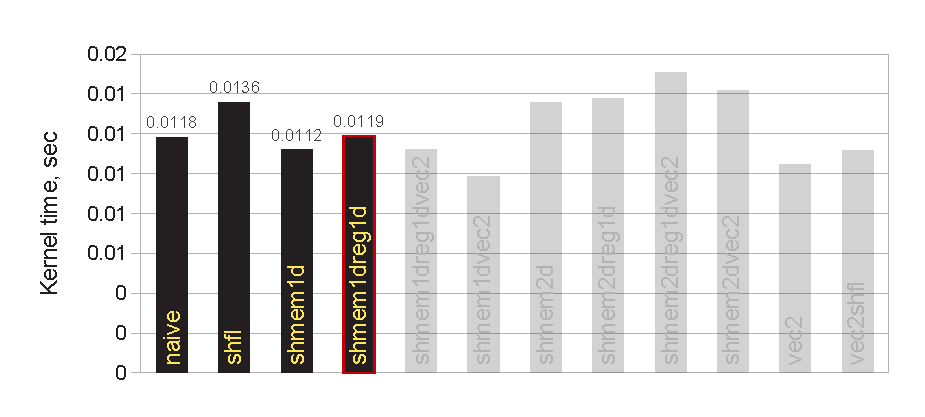
\includegraphics[width=7.5cm]{figures/wave13pt_time_04}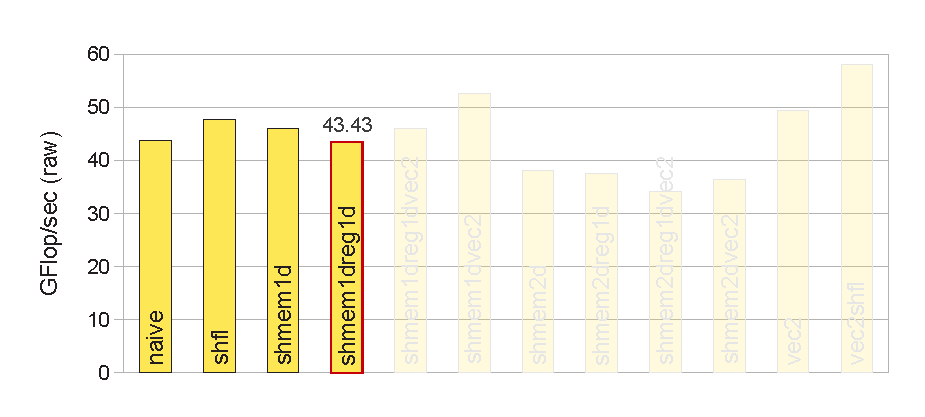
\includegraphics[width=7.5cm]{figures/wave13pt_gflops_04}};
\node [xshift=0cm,yshift=0cm] at (7.45cm,-3.85cm)
{\scriptsize \texttt{wave13pt} on GeForce GTX 680M (GK104/SM\_30), single precision};
\end{tikzpicture}%
\end{frame}



\begin{frame}[fragile,t]{1D line of \emph{w1} array in shmem, vertical line in regs, vector LD/ST}

\begin{minipage}[t][2.5cm]{\textwidth}
\begin{itemize}
\item $\{128, 1, 1\}$ blocks
\item maxrregcount=32
\item each thread is handling points of the same vertical column
\item array items reusable by the next point are tiled in registers
\item each thread handles two points, using 2-element vector load/stores (LD.64/ST.64)
\end{itemize}
\end{minipage}

\begin{tikzpicture}[overlay] 
\node [xshift=0cm,yshift=0cm] at (7.45cm,-2cm)
{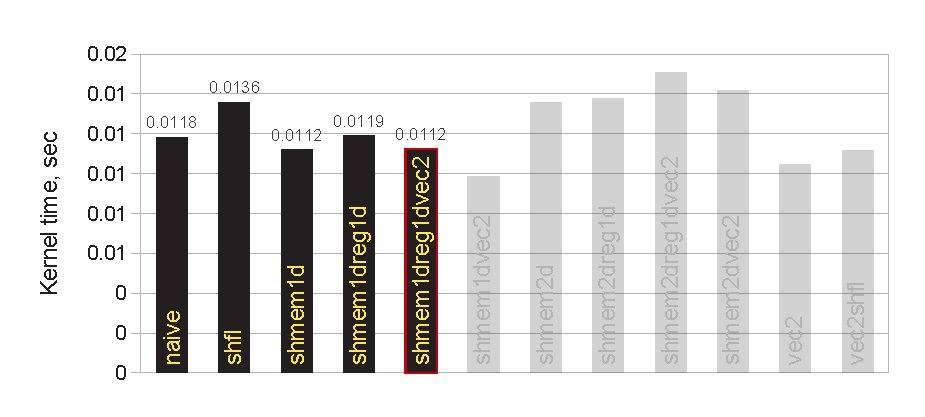
\includegraphics[width=7.5cm]{figures/wave13pt_time_05}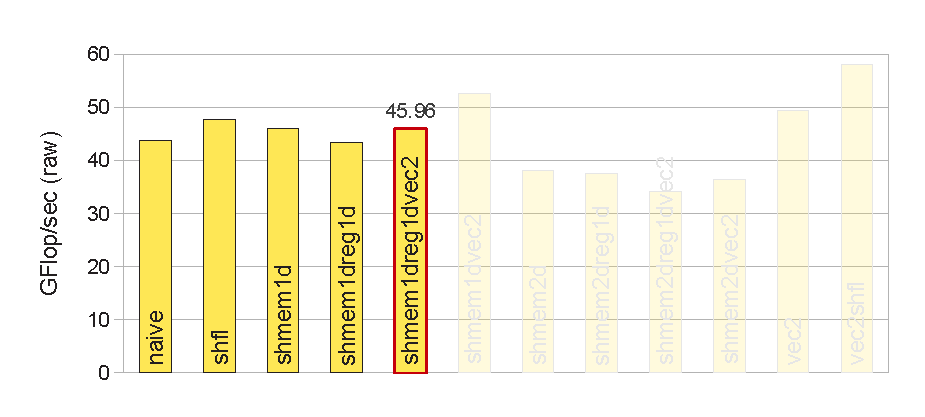
\includegraphics[width=7.5cm]{figures/wave13pt_gflops_05}};
\node [xshift=0cm,yshift=0cm] at (7.45cm,-3.85cm)
{\scriptsize \texttt{wave13pt} on GeForce GTX 680M (GK104/SM\_30), single precision};
\end{tikzpicture}%
\end{frame}



\begin{frame}[fragile,t]{1D line of \emph{w1} array in shmem, vector LD/ST}

\begin{minipage}[t][2.5cm]{\textwidth}
\begin{itemize}
\item $\{128, 1, 1\}$ blocks
\item maxrregcount=32
\item each thread handles two points, using 2-element vector load/stores (LD.64/ST.64)
\item[]
\end{itemize}
\end{minipage}

\begin{tikzpicture}[overlay] 
\node [xshift=0cm,yshift=0cm] at (7.45cm,-2cm)
{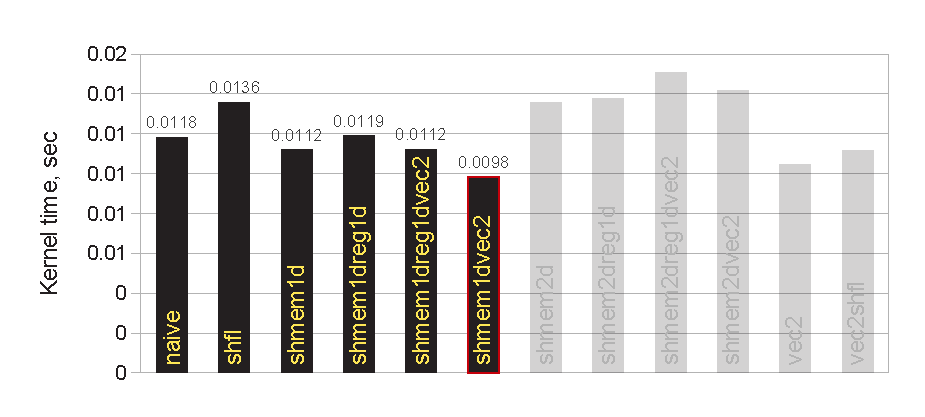
\includegraphics[width=7.5cm]{figures/wave13pt_time_06}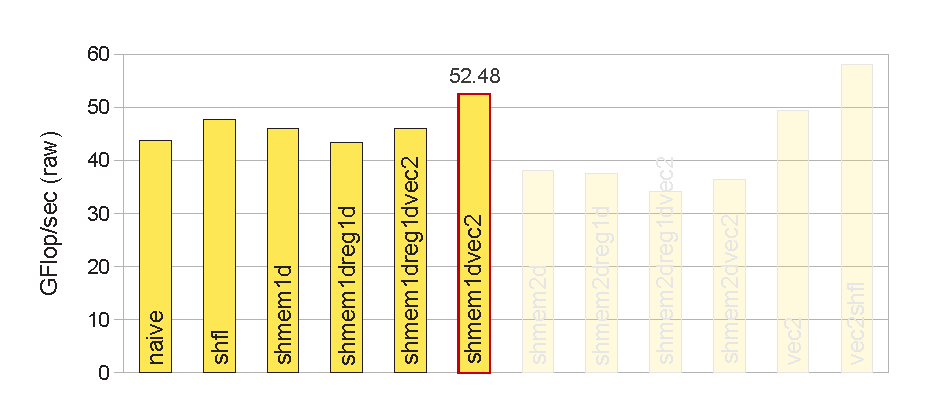
\includegraphics[width=7.5cm]{figures/wave13pt_gflops_06}};
\node [xshift=0cm,yshift=0cm] at (7.45cm,-3.85cm)
{\scriptsize \texttt{wave13pt} on GeForce GTX 680M (GK104/SM\_30), single precision};
\end{tikzpicture}%
\end{frame}




\begin{frame}[fragile,t]{Tiling 2D slice of \emph{w1} array in shmem}

\begin{minipage}[t][2.5cm]{\textwidth}
\begin{itemize}
\item[]
\item $\{32, 16, 1\}$ blocks
\item maxrregcount=32
\item \textcolor{blue}{additional time is spent on loading of shadow boundaries\\ by a subset of threads}
\end{itemize}
\end{minipage}

\begin{tikzpicture}[overlay] 
\node [xshift=0cm,yshift=0cm] at (7.45cm,-2cm)
{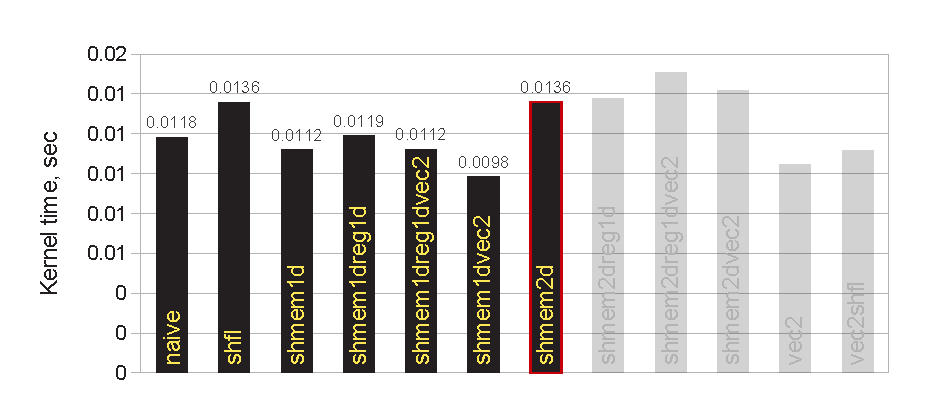
\includegraphics[width=7.5cm]{figures/wave13pt_time_07}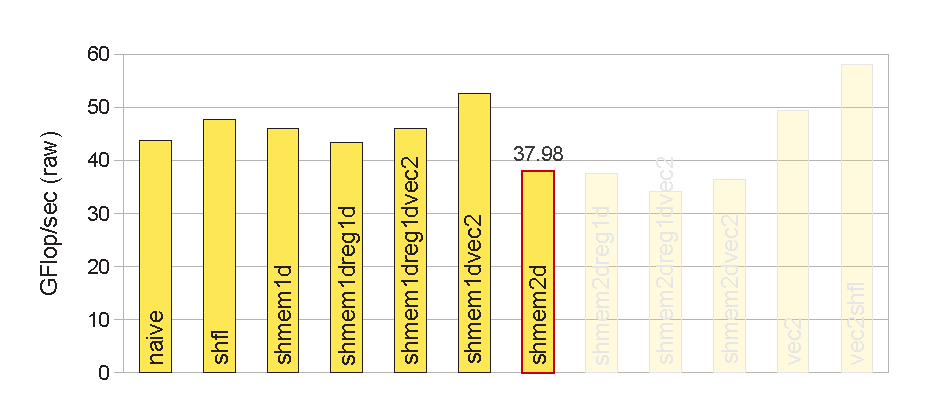
\includegraphics[width=7.5cm]{figures/wave13pt_gflops_07}};
\node [xshift=0cm,yshift=0cm] at (7.45cm,-3.85cm)
{\scriptsize \texttt{wave13pt} on GeForce GTX 680M (GK104/SM\_30), single precision};
\end{tikzpicture}%

\begin{tikzpicture}[overlay] 
\node [xshift=0cm,yshift=0cm] at (11.65cm,1.75cm)
{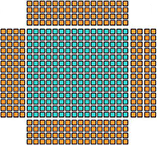
\includegraphics[width=2.5cm]{figures/paulius_fig1}};
\end{tikzpicture}
\end{frame}



\begin{frame}[fragile,t]{Tiling 2D slice of \emph{w1} array in shmem, vertical line in registers}

\begin{minipage}[t][2.5cm]{\textwidth}
\begin{itemize}
\item[]
\item $\{32, 16, 1\}$ blocks
\item maxrregcount=32
\item array items reusable by the next point are tiled in registers
\end{itemize}
\end{minipage}

\begin{tikzpicture}[overlay] 
\node [xshift=0cm,yshift=0cm] at (7.45cm,-2cm)
{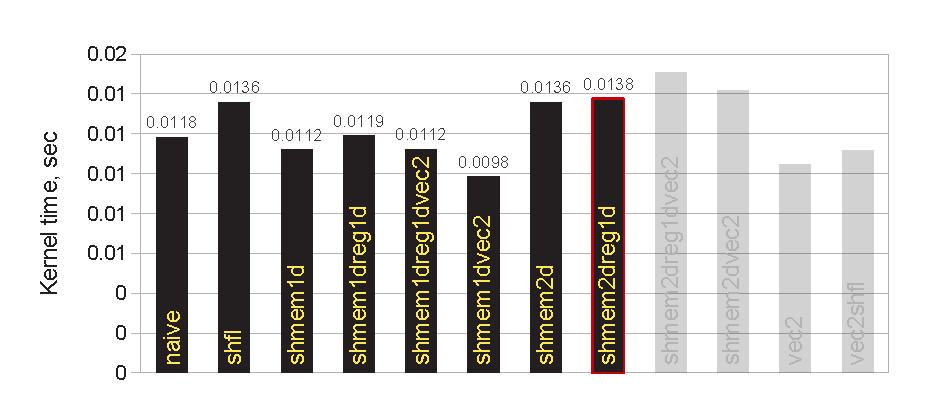
\includegraphics[width=7.5cm]{figures/wave13pt_time_08}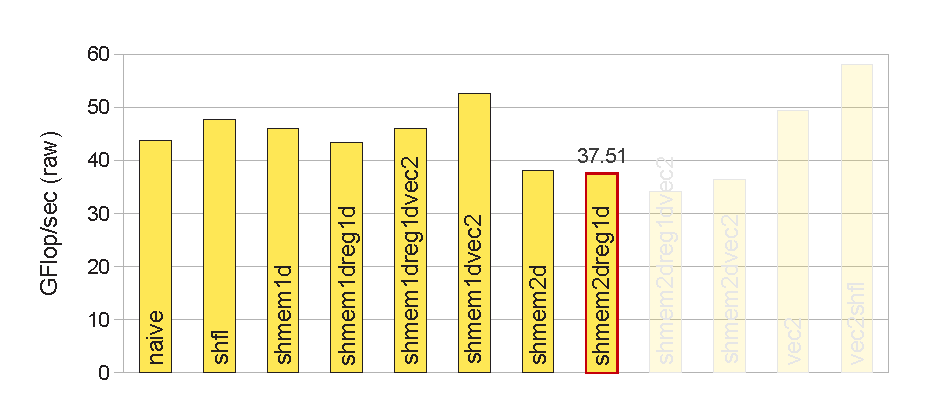
\includegraphics[width=7.5cm]{figures/wave13pt_gflops_08}};
\node [xshift=0cm,yshift=0cm] at (7.45cm,-3.85cm)
{\scriptsize \texttt{wave13pt} on GeForce GTX 680M (GK104/SM\_30), single precision};
\end{tikzpicture}%

\begin{tikzpicture}[overlay] 
\node [xshift=0cm,yshift=0cm] at (11.65cm,1.75cm)
{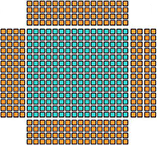
\includegraphics[width=2.5cm]{figures/paulius_fig1}};
\end{tikzpicture}
\end{frame}



\begin{frame}[fragile,t]{2D slice of \emph{w1} array in shmem, vertical line in regs, vector LD/ST}

\begin{minipage}[t][2.5cm]{\textwidth}
\begin{itemize}
\item[]
\item $\{32, 16, 1\}$ blocks
\item maxrregcount=32
\item array items reusable by the next point are tiled in registers
\item each thread handles two points, using 2-element vector load/stores (LD.64/ST.64)
\end{itemize}
\end{minipage}

\begin{tikzpicture}[overlay] 
\node [xshift=0cm,yshift=0cm] at (7.45cm,-2cm)
{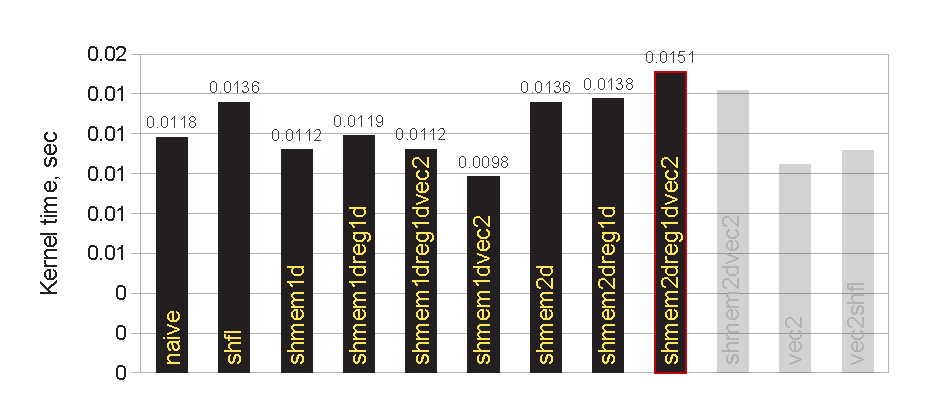
\includegraphics[width=7.5cm]{figures/wave13pt_time_09}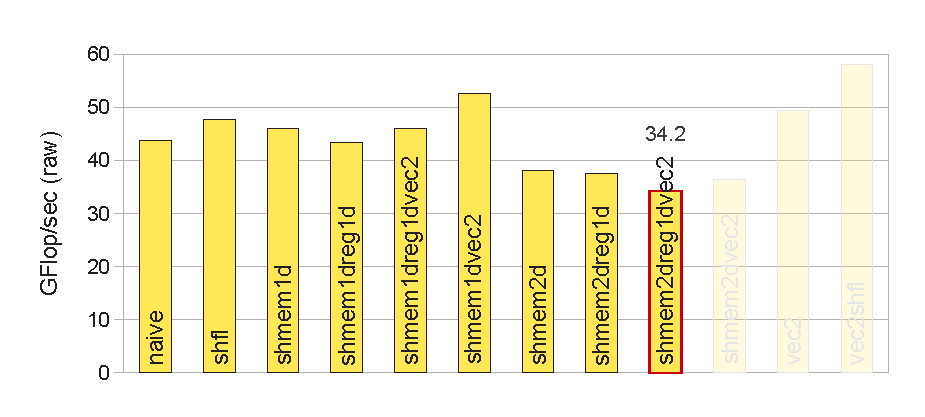
\includegraphics[width=7.5cm]{figures/wave13pt_gflops_09}};
\node [xshift=0cm,yshift=0cm] at (7.45cm,-3.85cm)
{\scriptsize \texttt{wave13pt} on GeForce GTX 680M (GK104/SM\_30), single precision};
\end{tikzpicture}%

\begin{tikzpicture}[overlay] 
\node [xshift=0cm,yshift=0cm] at (11.65cm,1.75cm)
{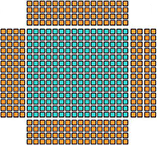
\includegraphics[width=2.5cm]{figures/paulius_fig1}};
\end{tikzpicture}
\end{frame}



\begin{frame}[fragile,t]{2D slice of \emph{w1} array in shmem, vector LD/ST}

\begin{minipage}[t][2.5cm]{\textwidth}
\begin{itemize}
\item[]
\item $\{32, 16, 1\}$ blocks
\item maxrregcount=32
\item each thread handles two points, using 2-element vector\\ load/stores (LD.64/ST.64)
\end{itemize}
\end{minipage}

\begin{tikzpicture}[overlay] 
\node [xshift=0cm,yshift=0cm] at (7.45cm,-2cm)
{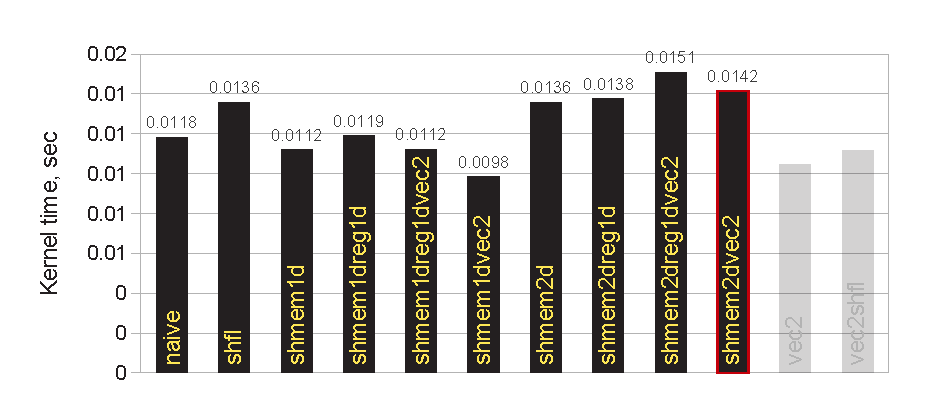
\includegraphics[width=7.5cm]{figures/wave13pt_time_10}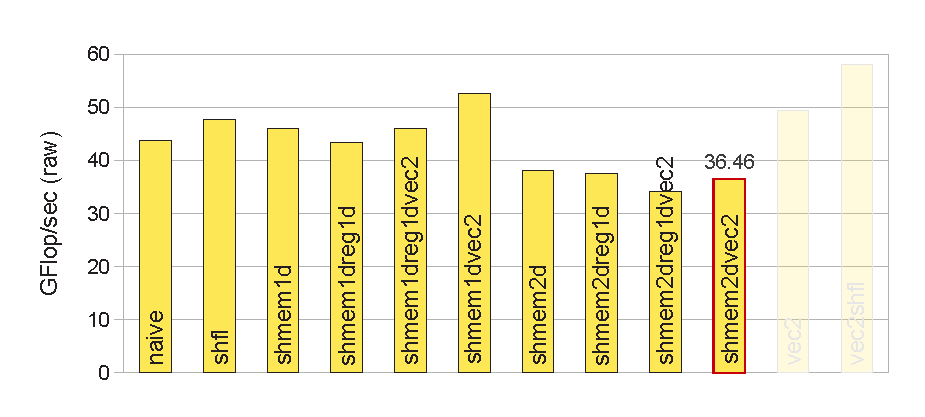
\includegraphics[width=7.5cm]{figures/wave13pt_gflops_10}};
\node [xshift=0cm,yshift=0cm] at (7.45cm,-3.85cm)
{\scriptsize \texttt{wave13pt} on GeForce GTX 680M (GK104/SM\_30), single precision};
\end{tikzpicture}%

\begin{tikzpicture}[overlay] 
\node [xshift=0cm,yshift=0cm] at (11.65cm,1.75cm)
{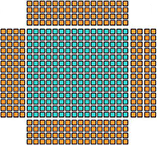
\includegraphics[width=2.5cm]{figures/paulius_fig1}};
\end{tikzpicture}
\end{frame}



\begin{frame}[fragile,t]{Vectorized load/store}

\begin{minipage}[t][2.5cm]{\textwidth}
\begin{itemize}
\item[]
\item[]
\item $\{128, 1, 1\}$ blocks
\item each thread handles two points, using 2-element vector load/stores (LD.64/ST.64)
\end{itemize}
\end{minipage}

\begin{tikzpicture}[overlay] 
\node [xshift=0cm,yshift=0cm] at (7.45cm,-2cm)
{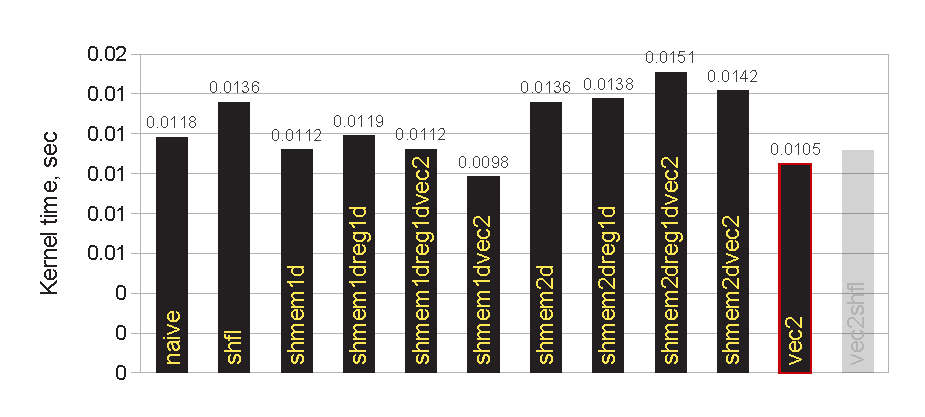
\includegraphics[width=7.5cm]{figures/wave13pt_time_11}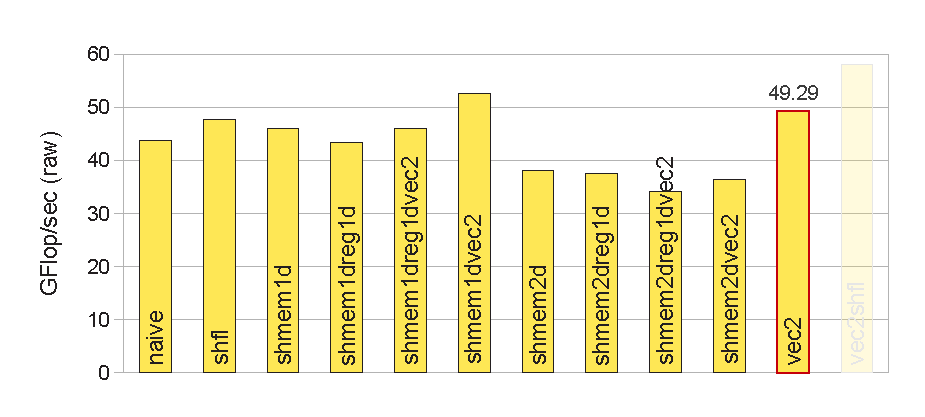
\includegraphics[width=7.5cm]{figures/wave13pt_gflops_11}};
\node [xshift=0cm,yshift=0cm] at (7.45cm,-3.85cm)
{\scriptsize \texttt{wave13pt} on GeForce GTX 680M (GK104/SM\_30), single precision};
\end{tikzpicture}%
\end{frame}



\begin{frame}[fragile,t]{Vectorized load/store, warp data shared with \emph{shuffle}}

\begin{minipage}[t][2.5cm]{\textwidth}
\begin{itemize}
\item $\{128, 1, 1\}$ blocks
\item each thread handles two points, using 2-element vector load/stores (LD.64/ST.64)
\item load array value, use and pass to neighboring thread
\item shuffles are accounted into FLOPS, hence more FLOPS, but larger kernel time
\item \textcolor{blue}{needs shareable flops to be beneficial}
\end{itemize}
\end{minipage}

\begin{tikzpicture}[overlay] 
\node [xshift=0cm,yshift=0cm] at (7.45cm,-2cm)
{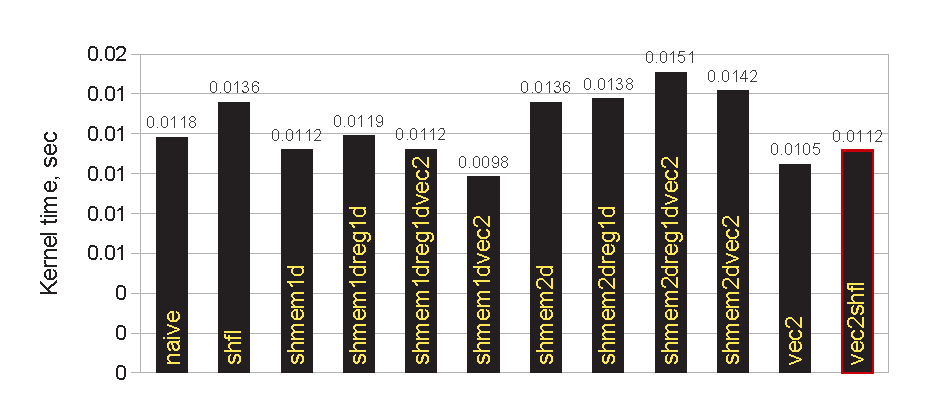
\includegraphics[width=7.5cm]{figures/wave13pt_time_12}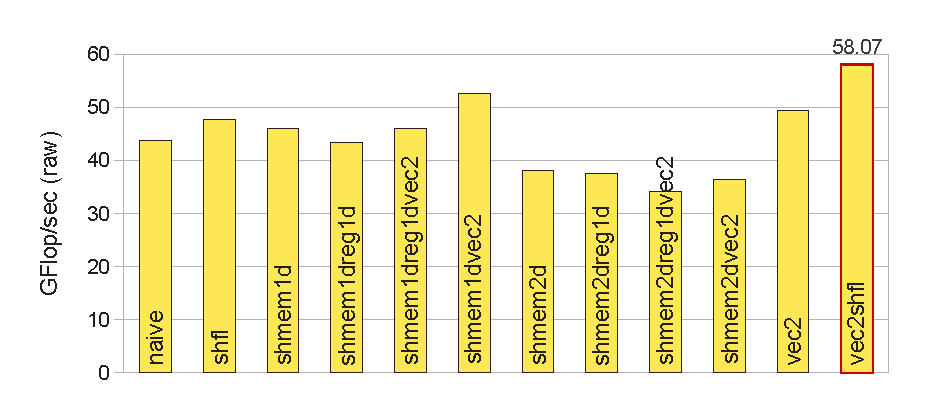
\includegraphics[width=7.5cm]{figures/wave13pt_gflops_12}};
\node [xshift=0cm,yshift=0cm] at (7.45cm,-3.85cm)
{\scriptsize \texttt{wave13pt} on GeForce GTX 680M (GK104/SM\_30), single precision};
\end{tikzpicture}%
\end{frame}



\begin{frame}[fragile,t]{The best manually-optimized version}

\begin{minipage}[t][2.5cm]{\textwidth}
\begin{itemize}
\item[]
\item 1D shared memory with vectorization is the best on GTX 680M
\item the contribution of shmem is minor
\item vectorization-only is the best on Tesla K20 (Piz Daint)
\item compared to {3$\times$} improvement on S1070, here tiling shows almost no speedup
\end{itemize}
\end{minipage}

\begin{tikzpicture}[overlay] 
\node [xshift=0cm,yshift=0cm] at (7.45cm,-2cm)
{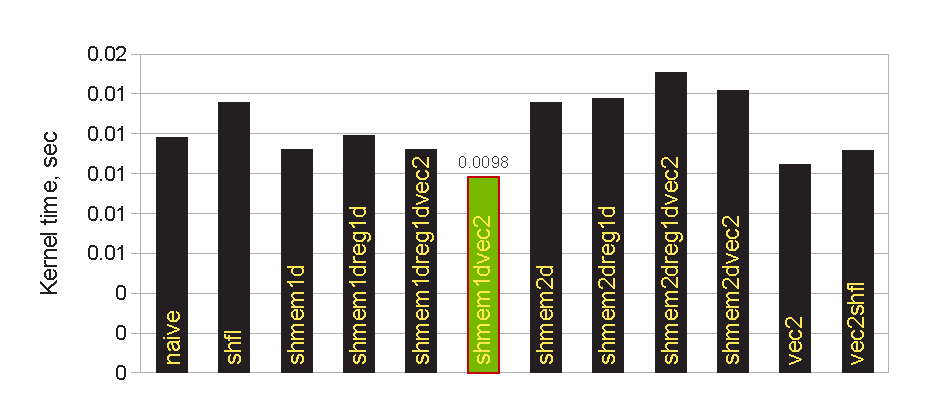
\includegraphics[width=7.5cm]{figures/wave13pt_time}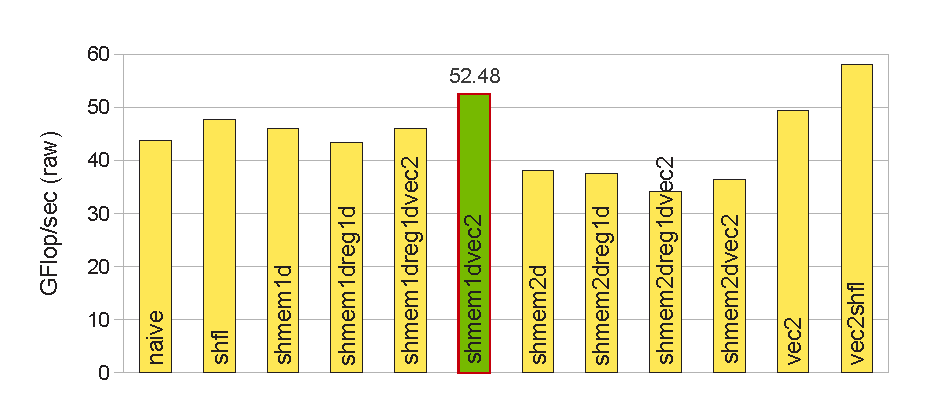
\includegraphics[width=7.5cm]{figures/wave13pt_gflops}};
\node [xshift=0cm,yshift=0cm] at (7.45cm,-3.85cm)
{\scriptsize \texttt{wave13pt} on GeForce GTX 680M (GK104/SM\_30), single precision};
\end{tikzpicture}%
\end{frame}



\begin{frame}[fragile]{What is the effect of vectorization at the low-level?}

\begin{itemize}
\item Surprisingly, the code of scalar kernel for memory-bound stencil appears to be compute-bound
\item 2-element vectorization improves the memory efficiency and reduces arithmetics (less indexing?)
\end{itemize}

\begin{center}
\begin{minipage}{6cm}
\begin{figure}
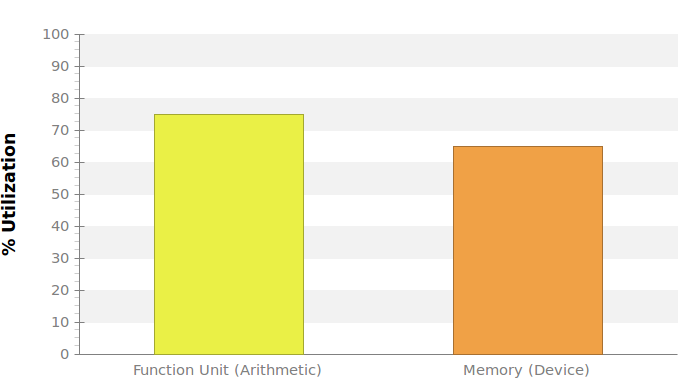
\includegraphics[width=6cm]{figures/cuda_utilization}
\caption{CUDA na\"{i}ve kernel}
\end{figure}
\end{minipage}%
\hskip1cm
\begin{minipage}{6cm}
\begin{figure}
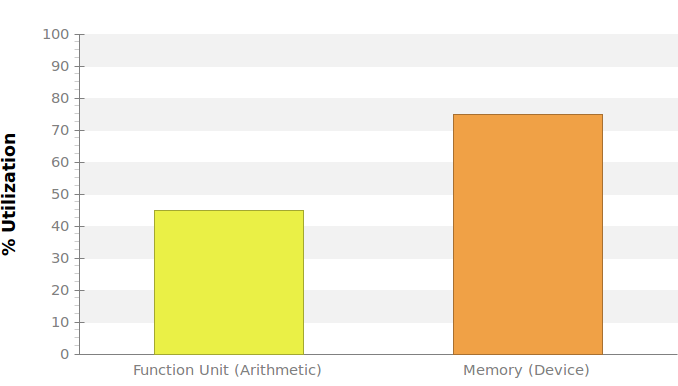
\includegraphics[width=6cm]{figures/cuda_vec2_utilization}
\caption{CUDA vectorized kernel}
\end{figure}
\end{minipage}
\end{center}

\end{frame}



\begin{frame}[fragile]{What is the effect of vectorization at the low-level?}

\begin{itemize}
\item Global memory throughput is higher in vectorized version\\ (very close to cuMemcpyDtoD, which is 84 Gb/sec on this device).
\end{itemize}

\begin{figure}
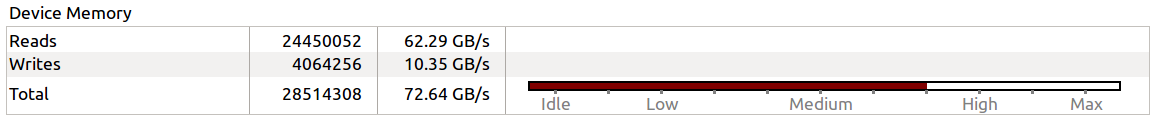
\includegraphics[width=11cm]{figures/cuda_gmem}
\caption{CUDA na\"{i}ve kernel}
\end{figure}
\vskip-25pt
\begin{figure}
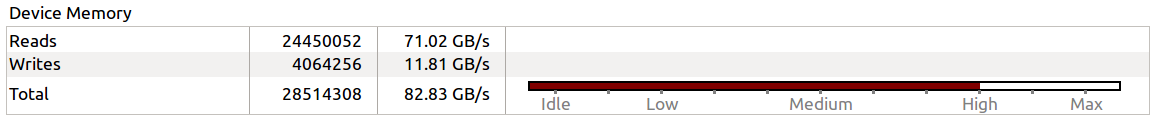
\includegraphics[width=11cm]{figures/cuda_vec2_gmem}
\caption{CUDA vectorized kernel}
\end{figure}

\end{frame}



\begin{frame}[fragile]{What is the effect of vectorization at the low-level?}

\definecolor{darkgreen}{rgb}{0,0.6,0}

\begin{itemize}
\item \textcolor{darkgreen}{kernel enjoys 4\% higher global memory load efficiency}
\item 13\% higher global store/write, 13\% higher global read and 7\% lower load throughput (less reloads to cache\textbf{?})
\item 13\% higher L2 write, 7\% lower L2 read, 7\% lower L2 read from L1 throughput
\item 40\% less used issue slots
\item 9\% less control-flow, 14\% less load-store instructions
\item 34\% higher instruction, 2.83$\times$ higher global memory replay overhead
\item 19\% less issued IPC, 45\% less instructions per warp
\item 58032 global stores, 84\% more global stores replayed due to divergence (\textbf{??})
\item \textcolor{red}{requires 1.5-2$\mathbin{\textcolor{red}{\times}}$ more registers per thread and may show no speedup in event of excessive spilling}
\end{itemize}

\end{frame}



\begin{frame}[fragile,t]{Another vectorization test on K20: tricubic}

\begin{minipage}[t][2.5cm]{\textwidth}
\begin{itemize}
\item[]
\item[]
\item Unlike \texttt{wave13pt}, \texttt{tricubic} test is compute-bound and has a large register footprint
\item No effect of vectorization on GTX 680M due to excessive register spilling
\item However, the same 12\% speedup is on Tesla K20, where the larger register file is available
\end{itemize}
\end{minipage}

\begin{tikzpicture}[overlay] 
\node [xshift=0cm,yshift=0cm] at (3.95cm,-2cm)
{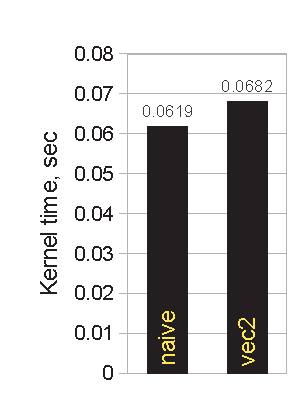
\includegraphics[width=2.4cm]{figures/tricubic_time_gtx680m}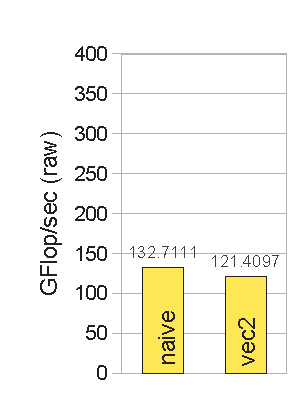
\includegraphics[width=2.4cm]{figures/tricubic_gflops_gtx680m}};
\node [xshift=0cm,yshift=0cm] at (3.95cm,-3.85cm)
{\scriptsize \texttt{tricubic} on GeForce GTX 680M (GK104/SM\_30), single precision};
\end{tikzpicture}%
\begin{tikzpicture}[overlay] 
\node [xshift=0cm,yshift=0cm] at (10.95cm,-2cm)
{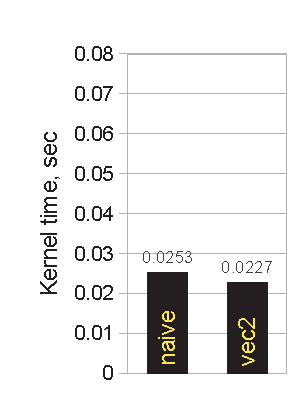
\includegraphics[width=2.4cm]{figures/tricubic_time_k20c}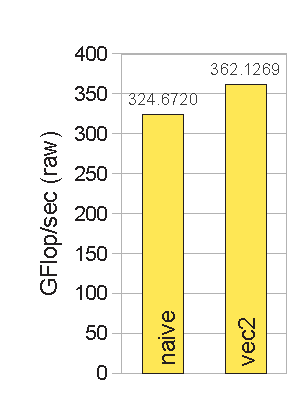
\includegraphics[width=2.4cm]{figures/tricubic_gflops_k20c}};
\node [xshift=0cm,yshift=0cm] at (10.95cm,-3.85cm)
{\scriptsize \texttt{tricubic} on Tesla K20 (GK110/SM\_35), single precision};
\end{tikzpicture}%
\end{frame}



\begin{frame}[fragile]{Extra minor observations}

\begin{itemize}
\item 13\% speedup with alignment of boundary threads:\\
\begin{minipage}{6.7cm}
\begin{lstlisting}[language=c, basicstyle=\tiny]
for (int k = 2+ k_start; k < ns - 2; k += k_inc)
    for (int j = 2 + j_start; j < ny - 2; j += j_inc)
        for (int i = 2 + i_start; i < nx - 2; i += i_inc)
        {
            ...
        }
\end{lstlisting}
\end{minipage}%
\hskip10pt$\Rightarrow$\hskip10pt
\begin{minipage}{6.5cm}
\begin{lstlisting}[language=c, basicstyle=\tiny]
for (int k = 2+ k_start; k < ns - 2; k += k_inc)
    for (int j = 2 + j_start; j < ny - 2; j += j_inc)
        for (int i = i_start; i < nx - 2; i += i_inc)
        {
            if (i < 2) continue;
        }
\end{lstlisting}
\end{minipage}
\item Caching in texture memory is enabled by default for noalias pointers (LDG instead of LD) on GK110. However, manual disabling of texture caching does not affect the perf.\\ $\Rightarrow$ Is it possible to create a tiling strategy making the texture cache beneficial for stencils?
\end{itemize}

\end{frame}



\begin{frame}[fragile]{Auto-parallelizing compilers}

\begin{itemize}
\item OpenACC
    \begin{itemize}
    \item Require a lot of manual assistance and introduce many practical limitations
    \end{itemize}
\item Polyhedral toolchains
    \begin{itemize}
    \item \textbf{PPCG} -- the newest polyhedral tool
        \begin{itemize}
        \item Transforms loops into parallel loops for execution on GPU
        \item Still requires manual tuning, without tuning is \textbf{10$\times$} slower than na\"{i}ve CUDA
        \item Clang frontend, then -- source-to-source
        \end{itemize}
    \item \textbf{KernelGen} -- a conservative descendant of \href{http://polly.llvm.org}{LLVM Polly}
        \begin{itemize}
        \item Checks loops for parallelism, assisted by runtime info and executes parallel loops on GPU
        \item Performs substitution of the runtime constants, reducing the register footprint at the price of JIT
        \item Default heuristics allow competitive performance, no tuning is needed
        \item GCC frontend, LLVM backend
        \end{itemize}
    \end{itemize}
\end{itemize}

\end{frame}



\begin{frame}[fragile]{{KernelGen} dependencies}

\begin{itemize}
\item \href{http://gcc.gnu.org/}{\bf GCC} -- for frontends and regular compiling pipeline \textcolor{blue}{(GPL)}
\item \href{http://dragonegg.llvm.org/}{\bf DragonEgg} -- GCC plugin for converting GCC's IR (gimple) into LLVM IR \textcolor{blue}{(GPL)}
\item \href{http://llvm.org/}{\bf LLVM} -- for internal compiler infrastructure \textcolor{blue}{(BSD)}
\item \href{http://polly.llvm.org/}{\bf Polly} -- for loops parallelism analysis \textcolor{blue}{(BSD+GPL)}
\item {\bf NVPTX backend} -- for emitting LLVM IR into PTX/GPU intermediate assembly \textcolor{blue}{(BSD)}
\item {\bf PTXAS} -- for emitting PTX/GPU into target GPU ISA \textcolor{blue}{(proprietary, no source code)}
\item \href{http://code.google.com/p/asfermi/}{\bf AsFermi} -- for necessary CUBIN-level tricks in Fermi GPU ISA \textcolor{blue}{(MIT/BSD)}
\item {\bf NVIDIA GPU driver} -- for deploying the resulting code on GPUs \textcolor{blue}{(proprietary, no source code)}
\item {\bf CUDA-aware \href{http://mvapich.cse.ohio-state.edu/overview/mvapich2/}{MVAPICH2}} -- for more efficient GPU peer-to-peer communication in {KernelGen}-{MPI} programs \textcolor{blue}{(BSD)}
\end{itemize}

\vskip 5pt

\end{frame}



\begin{frame}[fragile]{{KernelGen compiler pipeline}}

{KernelGen} conserves original host compiler pipeline (based on GCC), extending it with parallel LLVM-based pipeline, which is activated and/or used if specific environment variables are set.
\vskip 10pt
\setlength{\fboxsep}{0pt}%
\setlength{\fboxrule}{0.25pt}%
\begin{center}
\fbox{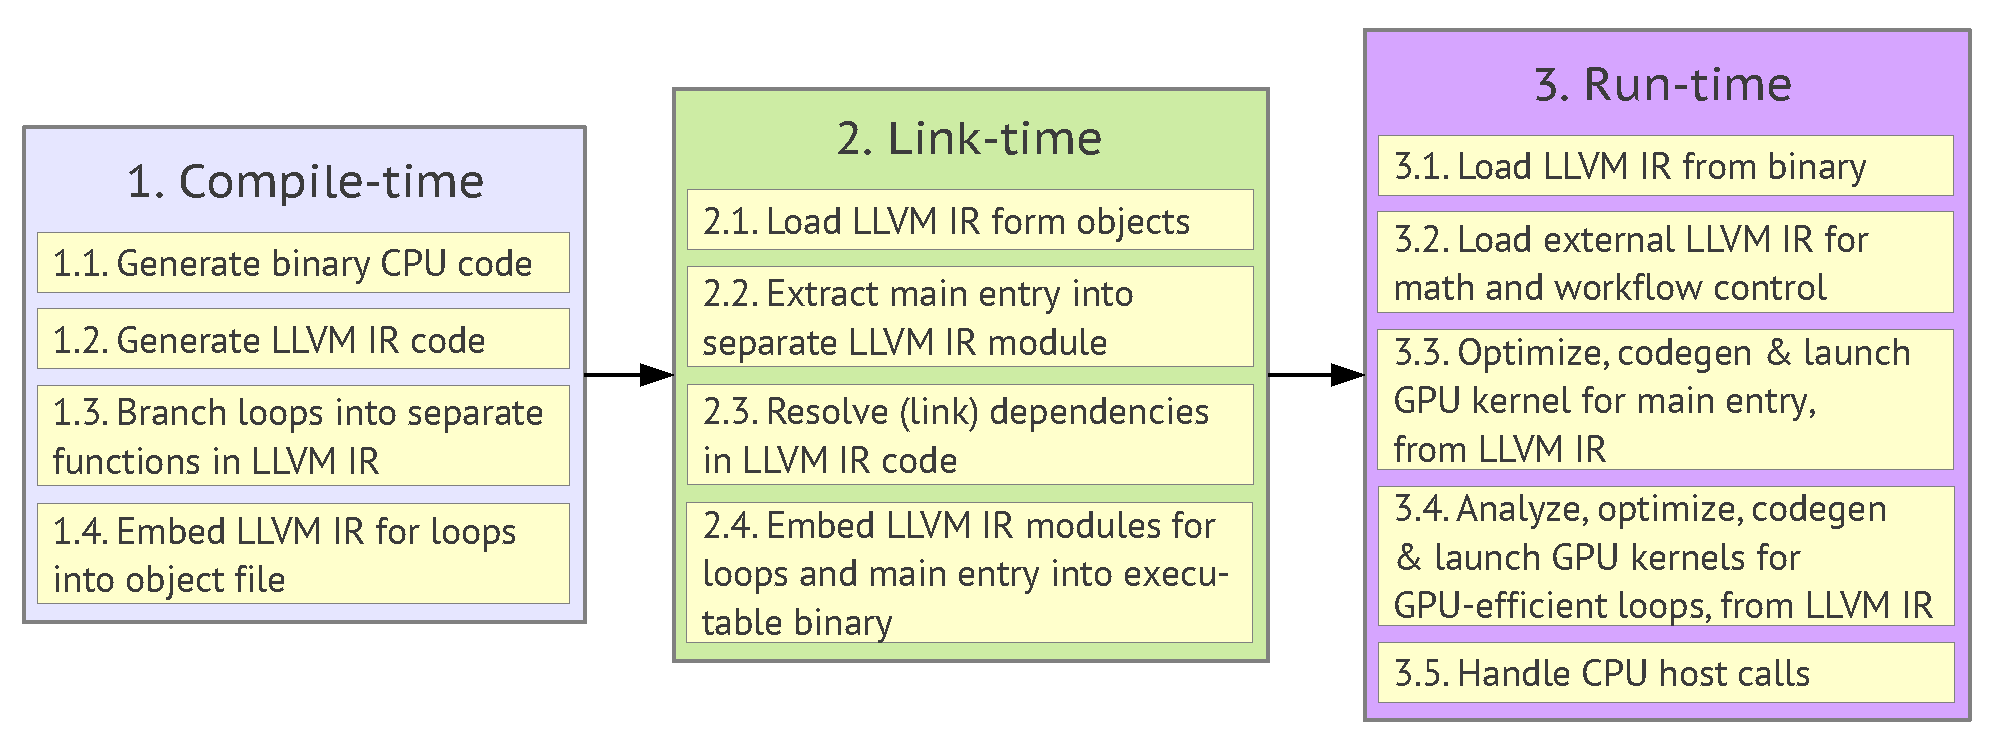
\includegraphics[height=5cm]{figures/code_generation_scheme}}
\end{center}

\end{frame}



\begin{frame}[fragile]{{{KernelGen} loops analysis pipeline}}

{KernelGen} takes part of loop analysis into runtime, in order to process only really used loops, and do it better with help of additional information available from the execution context. Introduced runtime overhead is neglectible, if the loop is invoked frequently. 
\vskip 10pt
\setlength{\fboxsep}{0pt}%
\setlength{\fboxrule}{0.25pt}%
\begin{center}
\fbox{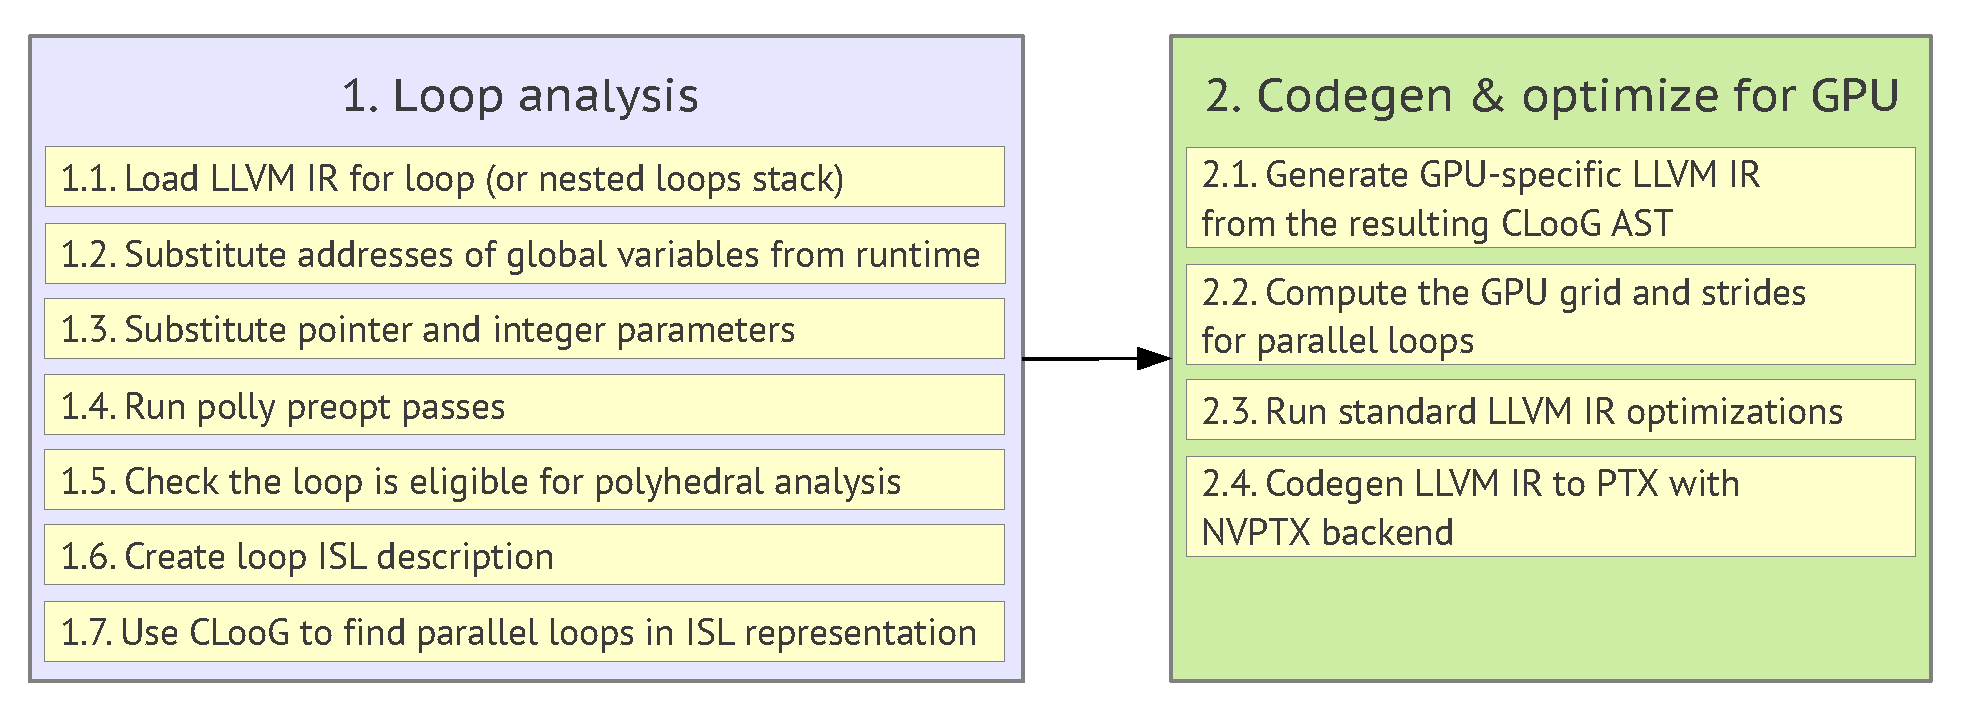
\includegraphics[height=4.5cm]{figures/polly_analysis_scheme}}
\end{center}

\end{frame}



\begin{frame}[fragile]{14-stencil test suite: benchmark}

{KernelGen} {\color{red}vs} {PGI OpenACC} {\color{red}vs} {CAPS OpenACC} on GTX 680

\begin{minipage}{10cm}
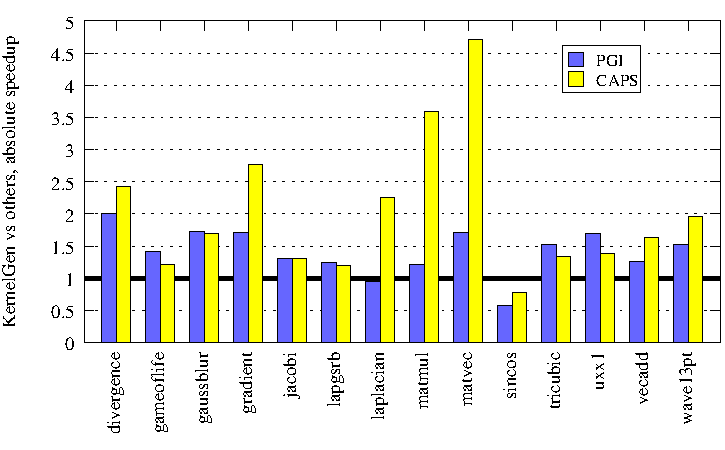
\includegraphics[width=10cm]{figures/intercomp_gtx680_single}
\end{minipage}%
\begin{minipage}{5cm}
{\footnotesize
\begin{itemize}
\item Tests precision mode: {\bf single}
\item Software: KernelGen r1780, PGI {OpenACC} 13.2, CAPS 3.2.4
\item Hardware: NVIDIA GTX 680 (GK104, sm\_30)
\item \textcolor{blue}{Speed-up values: \underline{above 1} -- KernelGen's kernel is faster than OpenACC's, \underline{below 1} -- OpenACC's kernel is faster than KernelGen's (on the same GPU)}
\item Measurements are averaged from 10 invocations of all tests and 10 iterations inside every test
\end{itemize}}
\end{minipage}

\end{frame}



\begin{frame}[fragile]{14-stencil test suite: roofline}

The test suite contains stencils with different arithmetic intensities:
\vskip3pt
\begin{minipage}{10cm}
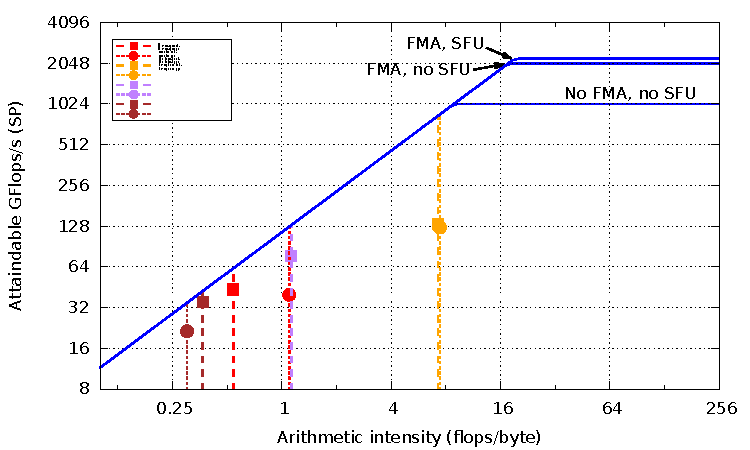
\includegraphics[width=10cm]{roofline_gtx680m}
\end{minipage}%
\begin{minipage}{5cm}
{\footnotesize
\begin{itemize}
\item Hardware: NVIDIA GTX 680M (GK104, sm\_30)
\end{itemize}}
\end{minipage}

\end{frame}



\begin{frame}[fragile]{Conclusions}

\begin{enumerate}
\item The most frequently cited shared memory optimizations are not beneficial\\ on modern cache-enabled GPUs
\item Vectorization of loads/stores gives 10-15\% improvement, and does not seem to be well-known\\ (the only prior reference is a recent brief \href{http://devblogs.nvidia.com/parallelforall/cuda-pro-tip-increase-performance-with-vectorized-memory-access/}{blog entry})
\item Compared to OpenACC commercial compilers, polyhedral toolchains can provide competitive performance for stencil codes
\item Open design toolchains could generate even better code with the new optimizations we've investigated
\item Yet to be addressed: how to efficiently transform for GPU codes with non-coalesced accesses in stencils
\end{enumerate}

\end{frame}



\begin{frame}[fragile]{Collaboration proposal}

\begin{itemize}
\item Joint implementation of vectorization and aligning in open-source polyhedral compiler
\vskip5pt
\item Joint work on tests, targets and optimizations research for a CUDA/OpenACC stencil benchmark:\\
\vskip10pt

\includegraphics[width=12cm]{figures/perfsuite}
\end{itemize}

\end{frame}



\usebackgroundtemplate%
{%
    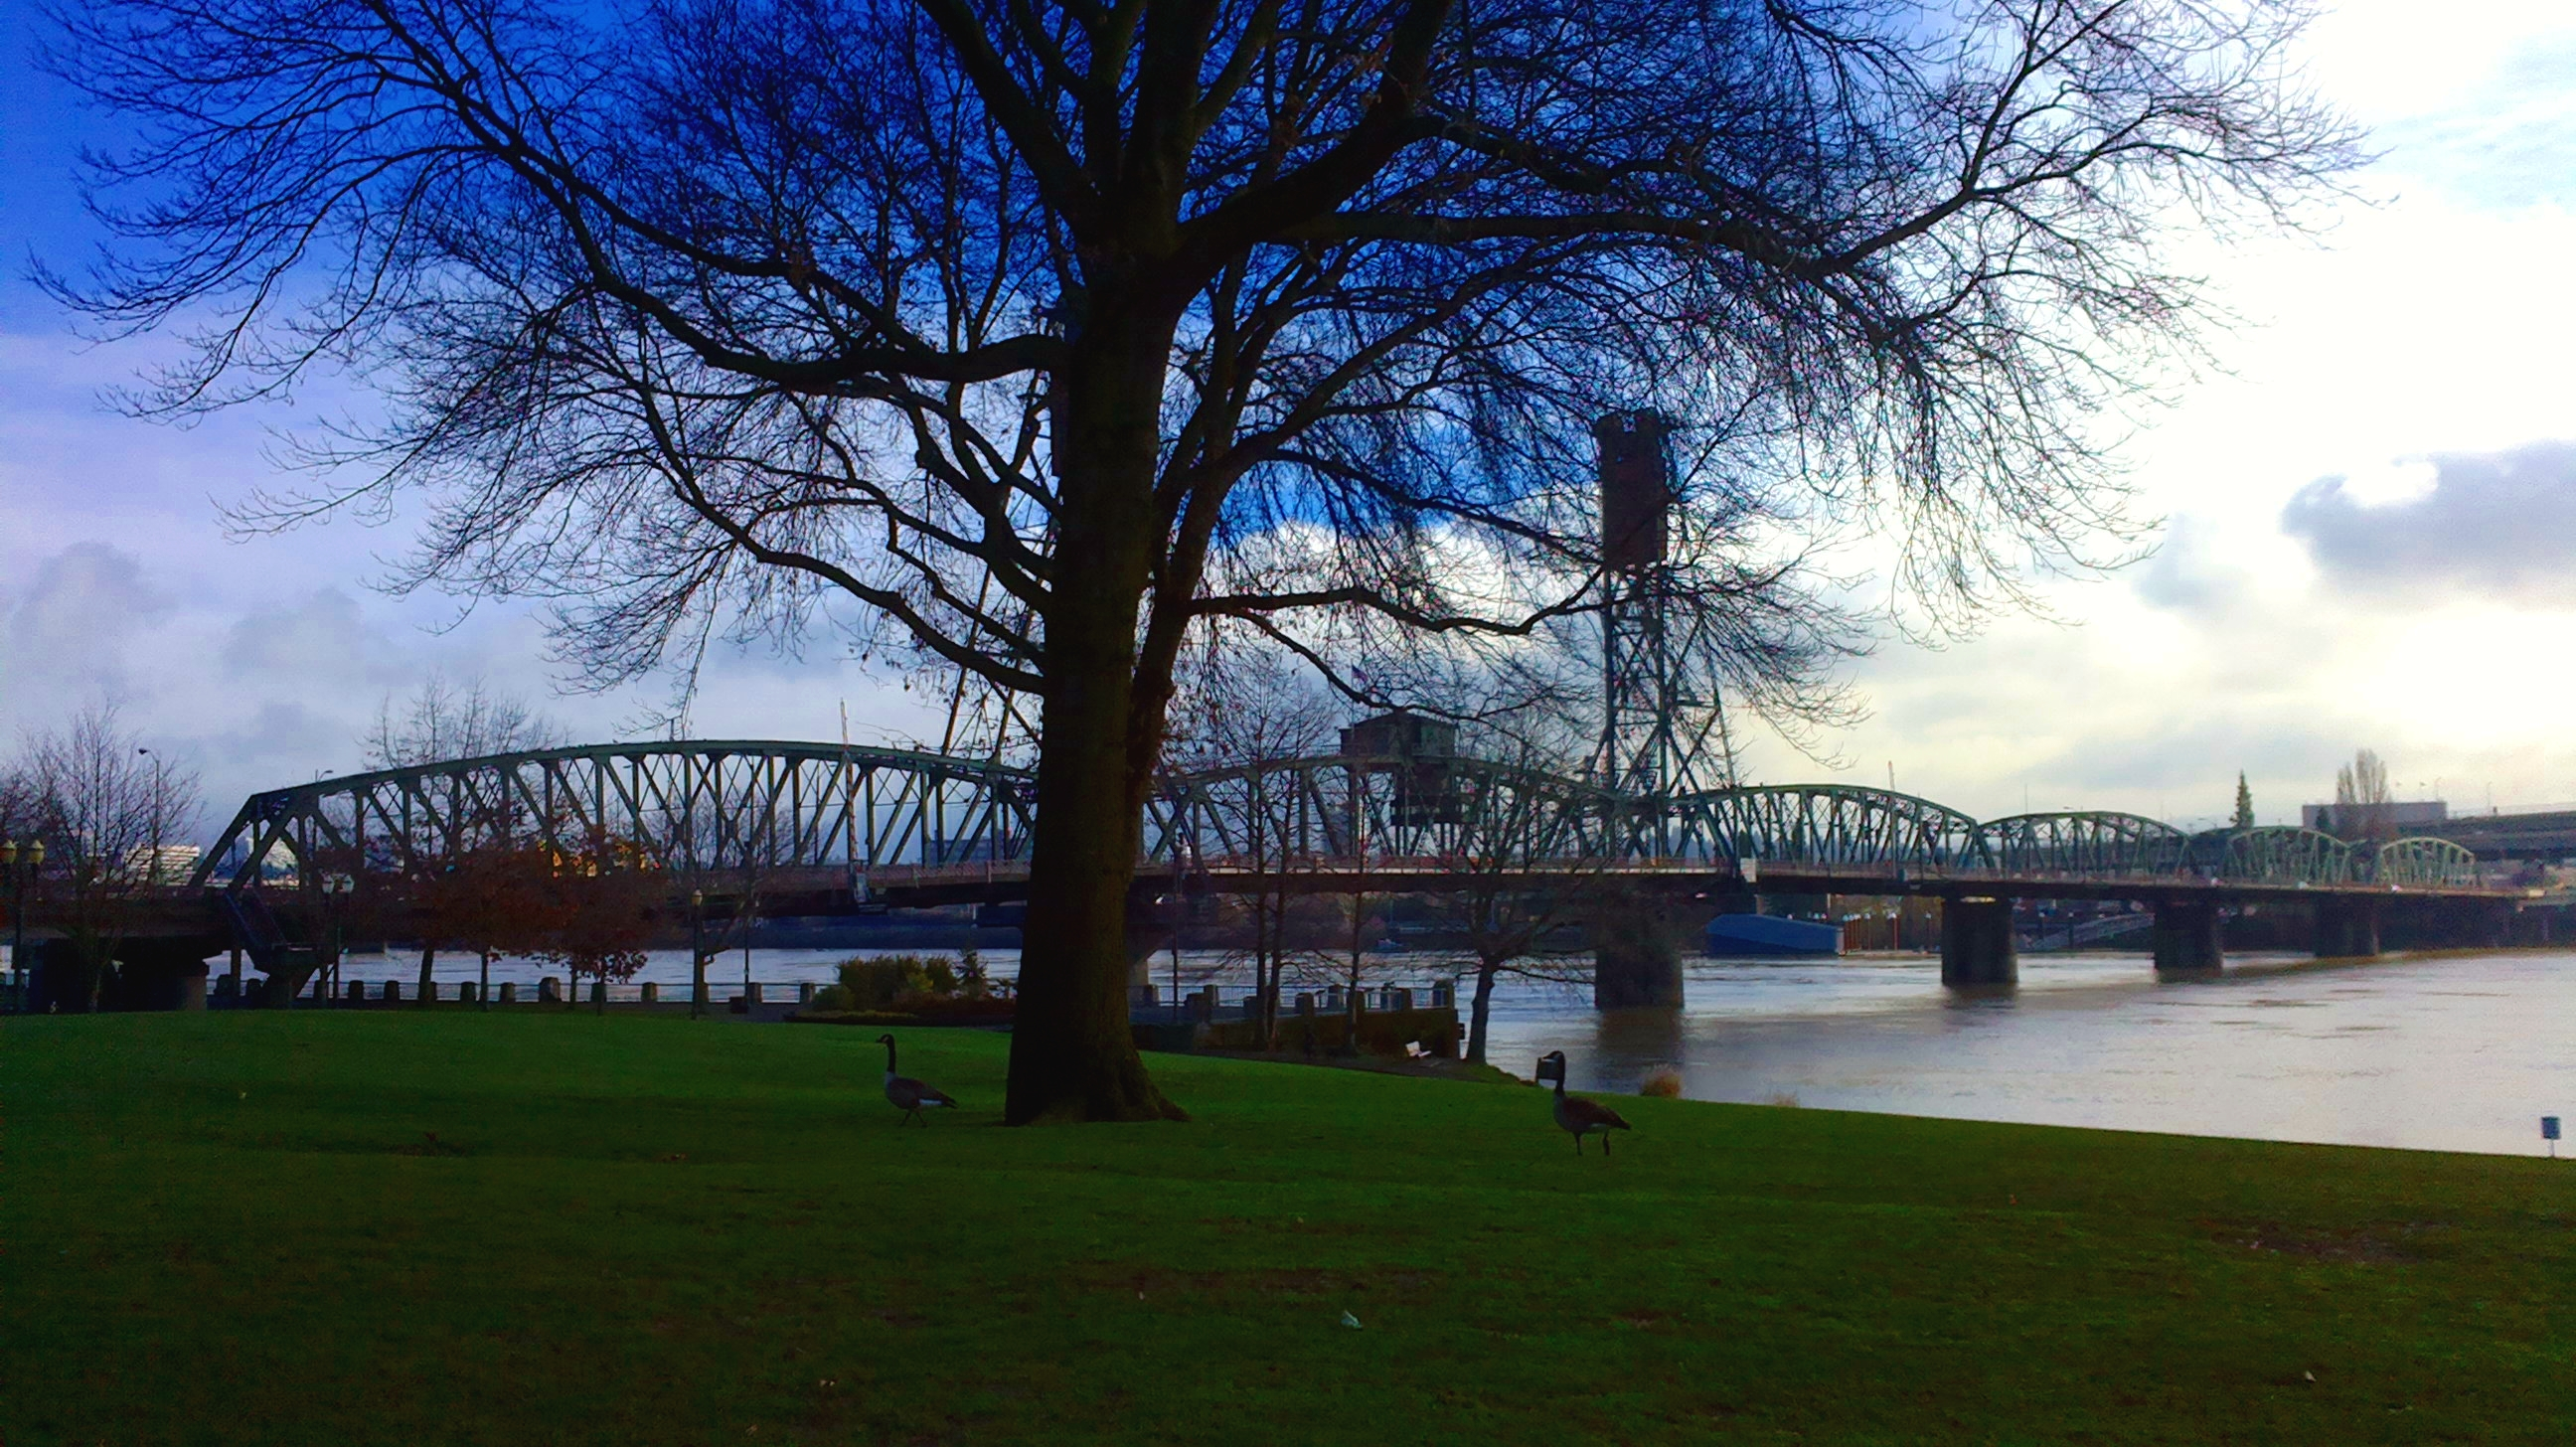
\includegraphics[width=\paperwidth,height=\paperheight]{figures/cover}%
}
\begin{frame}[fragile]{}

\vskip35pt
\begin{minipage}{0.38cm}
\hskip0.38cm
\end{minipage}%
\begin{minipage}{13cm}
\begin{center}
\textcolor{white}{\Huge \textbf{Thanks!}}
\end{center}
\vskip115pt
{\tiny
\begin{itemize}
\item[] \textcolor{white}{This presentation is supported by}
\item[] \textcolor{white}{\textbf{EXA2CT}: Exascale Algorithms and Advanced Computational Techniques (EU FP7-ICT programme)}
\vskip10pt
\item[] \textcolor{white}{Hardware access is provided by}
\item[] \textcolor{white}{\textbf{CSCS}: Swiss National Supercomputing Centre}
\item[] \textcolor{white}{\textbf{tesla-cmc}: GPU server @ Lomonosov Moscow State University}
\end{itemize}}
\end{minipage}
\end{frame}



\usebackgroundtemplate%
{%
}
\begin{frame}[fragile]{}

\begin{center}
\fbox{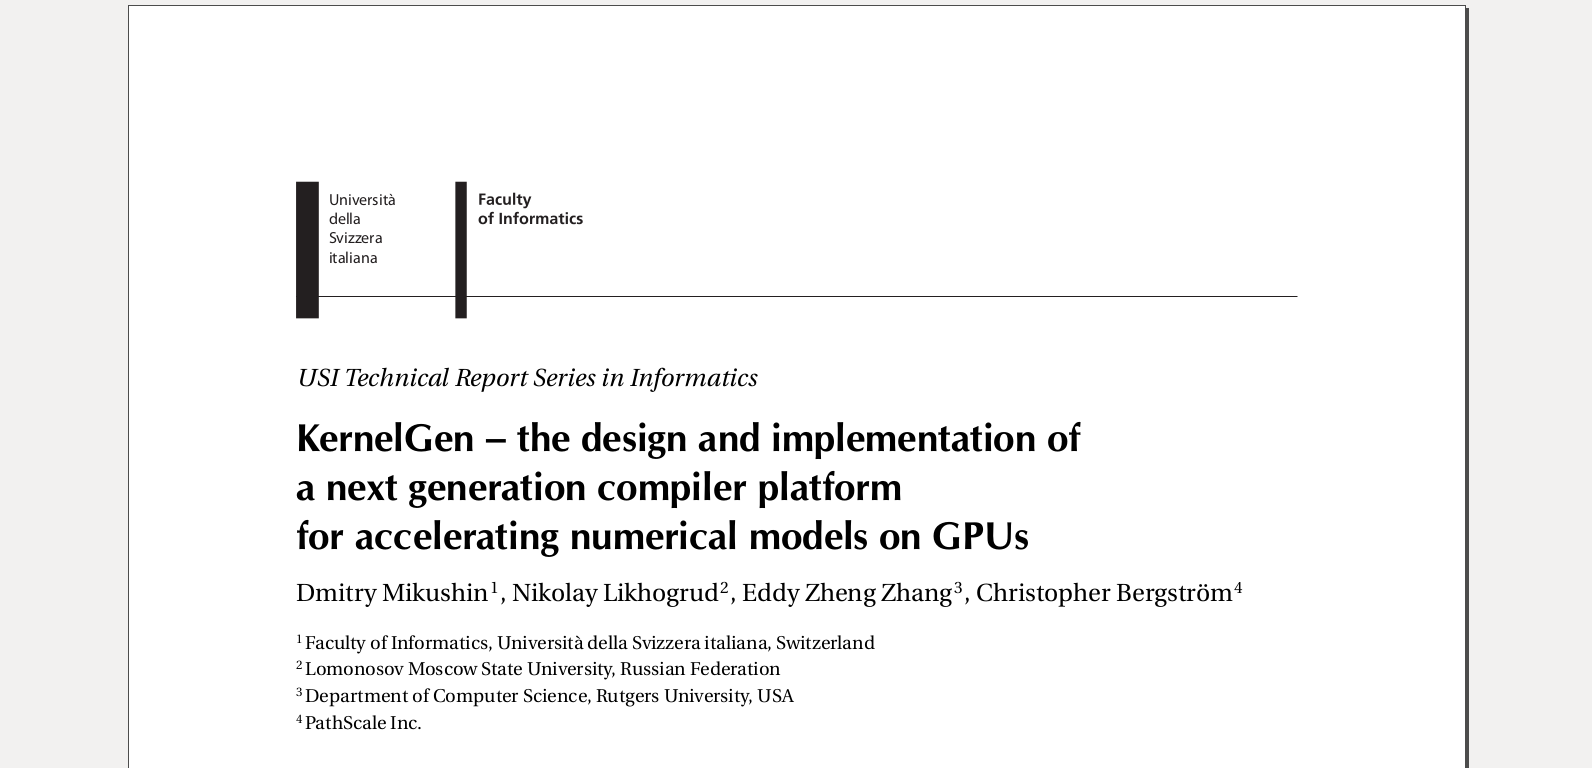
\includegraphics[width=13cm]{figures/techreport}}
\end{center}

\end{frame}

\end{document}
